\documentclass{article}
\usepackage{fullpage}
\usepackage{amssymb}
\usepackage{graphicx}
\begin{document}
\title{Stat 641 Project: Exponential and Gamma Distributions}
\author{Arthur Lui}
\maketitle
\def\wl{\par \vspace{\baselineskip}}


\section*{Introduction:}

  \subsection*{The Gamma Function:}
    The Gamma Function is defined as:
    \[
      \Gamma (\alpha) = \int\limits_0^\infty {t^{\alpha - 1} e^{-t} dt},
    \]
    where $\alpha > 0$.\\\\
   \subsection*{ Useful Identities:}
    \[
      \Gamma(\alpha+1) = \alpha\Gamma(\alpha), ~~~\alpha > 0
    \]
    \[
      \Gamma(n) = (n-1)!, ~~~ n ~ \epsilon ~ \mathbb{N}
    \]
    \[
      \Gamma(1) = 1
    \]
    \[
      \Gamma(\frac{1}{2}) = \sqrt(\pi)
    \]
  \subsection*{Derivation of the Gamma Distribution:}
     Consider
     \[
        f(t) = \frac{t^{\alpha-1} e^{-t}}{\Gamma(\alpha)},~~0~<~t~<\infty.
     \] 
     Integrating f(t) from $0~to~\infty$, we get
     \[
        \int\limits_0^\infty {f(t) dt} = 
        \int\limits_0^\infty {\frac{t^{\alpha - 1} e^{-t}}{\Gamma(\alpha)} dt} =
        \frac{\int\limits_0^\infty {t^{\alpha - 1} e^{-t}} dt}{\Gamma(\alpha)}
     \]
     \[
        = \frac{\Gamma(\alpha)}{\Gamma(\alpha)}
     \]
     \begin{equation} 
        = 1.
     \end{equation}
     Therefore, f(t) is a pdf. 

\section*{Derivation:}

  \subsection*{pdf:}
  Let $X \sim \beta T $ in (1), where $\beta > 0$. Then the $ gamma(\alpha,\beta) $ family is defined below as:
  \[
    f(x|\alpha,\beta) = \frac{1}{\Gamma(\alpha)\beta^\alpha}x^{\alpha-1}e^{-x/\beta}, ~~~ 0<x<\infty,~~~\alpha>0,~~~\beta>0.
  \]
  The parameters $\alpha$ and $\beta$ are referred to as the shape and scale parameters respectively as the $\alpha$ most influences the peakedness of the distribution, while $\beta$ most influenxes the spread of the distribution.

  \begin{center}
  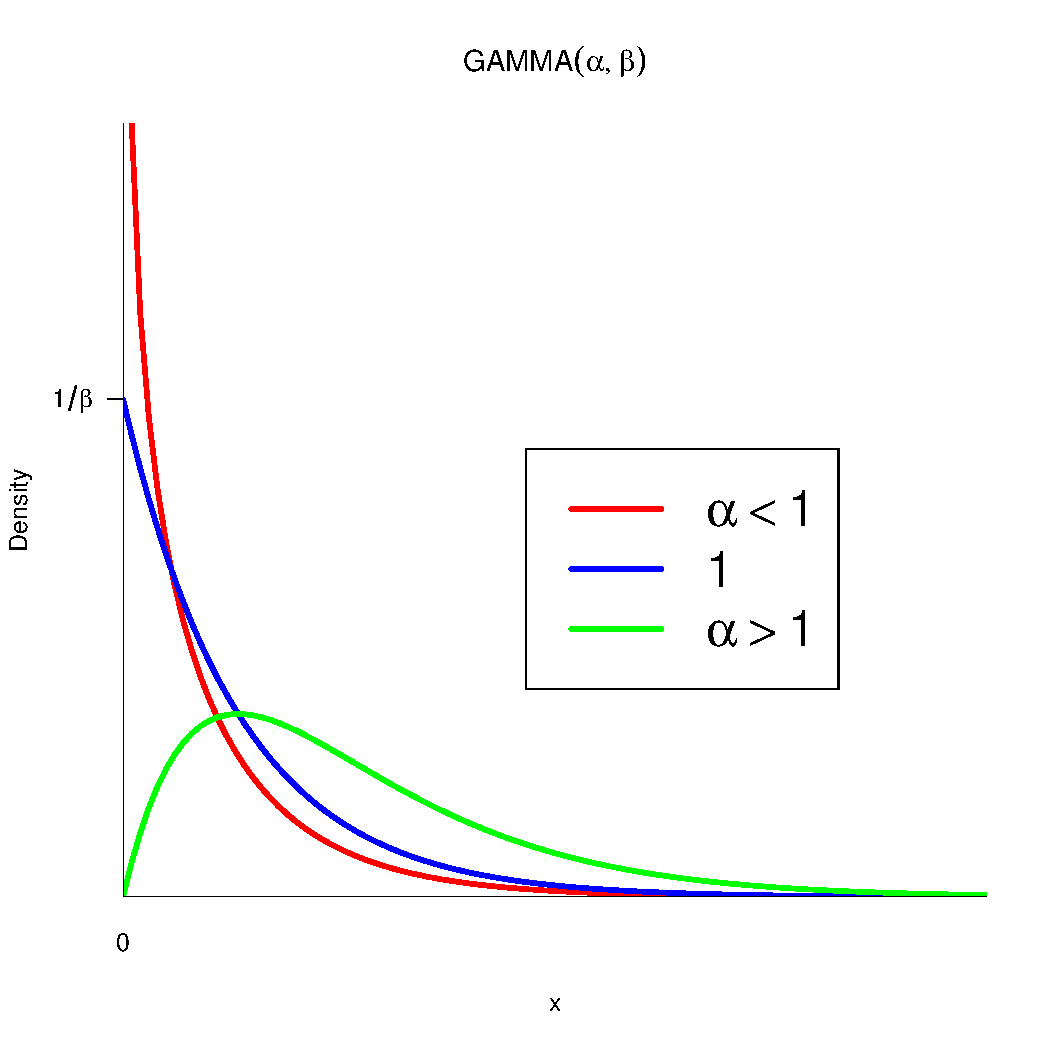
\includegraphics[scale=.5]{plot.pdf}
  \end{center}

  \subsection*{Integration to 1:}
  Let $X \sim \Gamma(\alpha,\beta)$, $x,\alpha,\beta > 0$. Then,
  \[
    \int\limits_0^\infty {f(x)dx}
  \]
  \[
    = \int\limits_0^\infty {\frac{1}{\Gamma(\alpha)\beta^\alpha}x^{\alpha-1}e^{-x/\beta}dx}
  \]
  \[
    = \frac{1}{\Gamma(\alpha) \beta^\alpha} \int\limits_0^\infty{x^{\alpha-1}e^{-x/\beta}dt}
  \]
  \[
    = \frac{\beta\beta^{\alpha-1}}{\Gamma(\alpha)\beta^\alpha} 
      \int\limits_0^\infty {\frac{x^{\alpha-1}}{\beta^{\alpha-1}}e^{-x/\beta}d\frac{x}{\beta}}
  \]
  \[
    = \frac{\beta^{\alpha}}{\Gamma(\alpha)\beta^\alpha}
      \int\limits_0^\infty
    { \left(\frac{x}{\beta}\right) ^ {\alpha-1} e^{-\frac{x}{\beta}} d\frac{x}{\beta}}
  \]
  \[
    = \frac{1}{\Gamma(\alpha)} \int\limits_0^\infty {t ^ {\alpha-1} e^{-t} dt}
  \]
  \[
    \frac{1}{\Gamma(\alpha)} \Gamma(\alpha) = 1.
  \]
  Therefore, f(x) integrates to 1. 
 
  \subsection*{CDF}
  The Gamma Cumulative Distribution is function is given by:
  \[
    \frac{\gamma(k,x/\theta)}{\Gamma(k)},
  \]
  where $k > 0$, and
  \[ 
    \gamma(k,x/\theta) = \int\limits_0^{x/\theta} {t^{k-1}e^{-t}dt}
  \]
  \section*{Mean and Variance:}
  \[
    E[X] = \alpha \beta 
  \]
  \subsection*{Proof:}
  \[
    E[X] = \int\limits_0^\infty {x\frac{1}{\Gamma(\alpha)\beta^\alpha}
                                 x^{\alpha-1} e^{-x/\beta} dx}
  \]
  \[
    = \frac{\Gamma(\alpha+1)\beta^{\alpha+1}}{\Gamma(\alpha)\beta^\alpha} 
      \int\limits_0^\infty {
        \frac{1}{\Gamma(\alpha+1)\beta^{\alpha+1}} 
        x^{\alpha+1} e^{-x/\beta}
      dt}
  \]
  \[
    = \frac{\Gamma(\alpha+1)\beta^{\alpha+1}}{\Gamma(\alpha)\beta^\alpha}
  \]
  \[
    = \frac{\Gamma(\alpha+1)}{\Gamma(\alpha)}\beta
  \]
  \[
    = \frac{\alpha\Gamma(\alpha)}{\Gamma(\alpha)}\beta
  \]
  \[
    = \alpha\beta
  \]
  \wl
  \[
    Var[X] = \alpha \beta^2
  \]
  \subsection*{Proof:}
  \[
    E[X^2] = \int\limits_0^\infty {x^2\frac{1}{\Gamma(\alpha)\beta^\alpha}
                                 x^{\alpha-1} e^{-x/\beta} dx}
  \]
  \[
    = \frac{1}{\Gamma(\alpha)\beta^{\alpha}} 
      \int\limits_0^\infty { x^{(\alpha+2)-1} e^{-x/\beta}dx}
  \]
  \[
    \frac{\Gamma(\alpha+2)\beta^{\alpha+2}}{\Gamma(\alpha)\beta^{\alpha}}
  \]
  \[
    = (\alpha+1)\alpha\beta^2
  \]
  \wl
  Therefore,
  \[
    Var[X] = E[X^2] - (E[X])^2
  \]
  \[
    =(\alpha+1)\alpha\beta^2 - (\alpha\beta)^2
  \]
  \[
    = \alpha\beta^2
  \]
  \section*{Moment Generating Function:}
  \[
    M_x(t) = E[e^{tx}] = {\left( \frac{1}{1-\beta^t} \right)} ^ \alpha
  \]
  \[
    M_x(t) = \int\limits_0^\infty { e^{tx} \frac{1}{\Gamma(\alpha)\beta^\alpha} 
                                    e^{-x/\beta} x^{\alpha-1}dx}
  \]
  \[
    = \int\limits_0^\infty { \frac{1}{\Gamma(\alpha)\beta^\alpha} 
                             e^{-(x/\beta) + tx}x^{\alpha-1}dx}
  \]
  \[
    = \frac{1}{\beta^\alpha} \int\limits_0^\infty { 
      \frac{ \left( {\frac{1}{(1/\beta)-t}} \right)^\alpha } 
            {\left( \Gamma(\alpha){\frac{1}{(1/\beta)-t}} \right) ^\alpha}
      e^{-x/\frac{1}{(1/\beta)-t} } x ^ {\alpha-1} dx}
  \]
  \[
    = \left( {\frac{1}{(1/\beta)-t}} \right)^\alpha / \beta^\alpha
  \]
  \[
    = \left( {\frac{1}{[(1/\beta)-t]\beta}} \right)^\alpha
  \]
  \[
    = \left( \frac{1}{1-\beta t}\right) ^ \alpha
  \]

  \subsection*{Relation to Other Distributions:}
  \textbf{Poisson-Gamma.} The Gamma distribution is a conjugate prior
  for the mean of the Poisson distribution.\\
  \textbf{Exponential-Inverse Gamma.} The Inverse Gamma distribution is a
  conjugate prior for the mean of the exponential distribution. \\
  \wl
  \textbf{Exponential.} $Gamma(1,\beta) = EXP(\beta)$.\\
  \textbf{Chi-Sqaured.} $Gamma(p/2,2) = \chi ^2 (p)$.\\
  \textbf{Maxwell.} Let X be distributed as a Gamma. If $\alpha = 3/2$, then $Y = \sqrt{X/\beta}$ is distributed as a Maxwell.\\
  \textbf{Inverse Gamma.} Let $X \sim Gamma(\alpha,\beta)$. Then $Y = 1/X \sim InverseGamma(\alpha,\beta)$.\\
  \wl
  \textbf{More on Poisson-Gamma.} The Negative Binomial can be derived as a gamma mixture of Poissons.\\
  \wl
  Specifically, if
  \[
     X \sim NB (r,\beta)
  \]
  and
  \[
    X|\lambda \sim POI(\lambda),
  \]
  then
  \[
    \lambda \sim Gamma(r,\beta).
  \]


  \subsection*{Applications of the Gamma Distribution:}
  The Gamma distribution is positive and right-skewed, so it is can be used to model a variety of events, including the following:
    \wl
    \wl
    - The amount of rainfall accumulated in a reservoir\\
    - The size of loan defaults of aggregate insurance claims\\
    - The flow of items through manufacturing and distribution processes\\
    - The load on web servers\\
    - The many and varied forms of telecom exchange

  \subsection*{Example:}
  Suppose that for a graduate Statistical Computing course, the average time required for every student to come up with a feasible solution for each exam problem is two hours. Compute the probability that a student, say Mickey, will take 8 or more hours to come up with the solutions to all four problems of the exam.\\
\wl
One problem every 2 hours means we would expect to "solve" $\beta = 1/2$ exam problems every hour on average. Using $\beta = 1/2 $ and $\alpha = 16$, we can compute this as follows:
\[
  P(X \ge 8) = \int\limits_8^\infty {\frac{x^{16-1}e^{-x/.5}}{\Gamma(16)(1/2)^{16} }dx}
             = .466745
\]


\end{document}


